\documentclass[varwidth,convert={density=500,size=1080x800,outext=.png}]{standalone}
\usepackage{mathtools}
\usepackage{graphicx}
\usepackage{bm}
\usepackage{color}
\usepackage[dvipsnames,table]{xcolor}
\usepackage{tikz}
\usepackage{stanli}
\usepackage{verbatim}
\usepackage{tikz}
\usetikzlibrary{shapes,calc,through,3d,patterns}
\usetikzlibrary{decorations.pathreplacing}
\usepackage{pgfplots}
\usepackage{siunitx} % For formatting numbers
\usepackage{hyperref}
\hypersetup{colorlinks=true,linkcolor=darkred}
\usepackage{multicol}
\usepackage[absolute,overlay,]{textpos}
\usepackage{pgfplots}
\pgfplotsset{width=10cm,compat=1.9}
\usepackage{subcaption}
\usepackage{multirow}
\usepackage{bbding}
\usepackage{arydshln}
\usepackage{mathtools}
\usepackage{tcolorbox}

\usepackage[dvipsnames]{xcolor}

\begin{document}
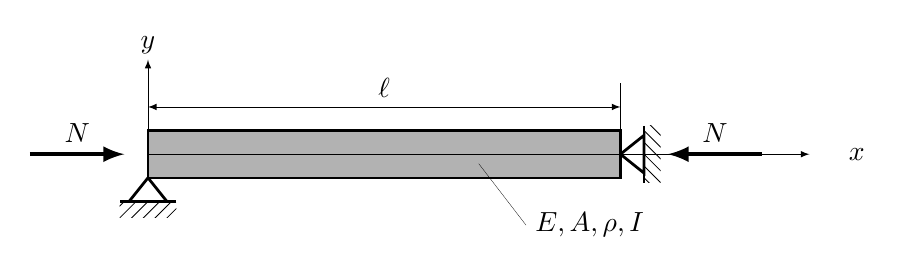
\begin{tikzpicture}[scale=0.6]
      \point{a}{0}{0};
      \point{b}{6}{0.3};
      \support {1}{a}[0];
      \support {1}{b}[90];
      % Draw the rectangle
      \filldraw[fill=gray!60, draw=black,thick] (0,0) rectangle (10,1);
      %axis
      \draw[-latex, ultra thin] (0,0.5) -- (14,0.5);
      \draw[-latex, ultra thin] (0,0) -- (0,2.5);
      \node at (15,0.5) {\(x\)};
      \node at (0,2.8) {\(y\)};
      % length
      \draw[ultra thin] (10,0) -- (10, 2) ;
      \draw[latex-latex, ultra thin]  (0,1.5)  to node[sloped,midway,above] {$\ell$}(10,1.5) ;
      % N
      \draw[latex-, ultra thick] (11,0.5) -- (13,0.5) node[midway, above]{$N$};
      \draw[-latex, ultra thick] (-2.5,0.5) -- (-0.5,0.5) node[midway, above]{$N$};
      \draw[ultra thin]  (7,0.3) -- (8,-1) node[right]{$E,A,\rho,I$};
    \end{tikzpicture}
\end{document}